\chapter{Problema della Fermata e Funzione Universale}

\section{Concetti Introduttivi Generali}

Fino ad adesso ci siamo concentrati sul concetto di calcolabilità e sulla descrizione delle proprietà delle funzioni calcolabili.

Per quanto siamo riusciti a ottenere ottimi risultati nel caratterizzarle, non siamo ancora riusciti a trarre conclusioni di carattere generale sulle funzioni calcolabili.

In questo capitolo procederemo a trattare due dei più importanti risultati dell'informatica teorica che vanno in questo senso, ovvero il \textbf{problema della fermata e l'esistenza di funzioni non calcolabili} e la \textbf{funzione universale}.

Il primo dei due risultati risponde alla domanda se \textbf{esistono funzioni che non possono essere risolti da un algoritmo}, mentre il secondo risponde alla domanda \textbf{se esiste un algoritmo che può risolvere ogni problema risolvibile}.

Per quanto possano sembrare formulazioni molto simili, andremo a dimostrare come nel primo caso otterremo un risultato \textbf{in senso negativo}, mentre nel secondo un risultato \textbf{in senso positivo}.

Prima di fare ciò però è fondamentale introdurre degli ultimi strumenti utili che ci permetteranno di dimostrare questi risultati, ovvero la \textbf{funzione di pairing} e i \textbf{numeri di Gödel}, che ci permetteranno di procedere alla \textbf{codifica dei programmi in numeri}, fondamentale per permettere a degli algoritmi di valutarli.

\newpage
\section{Funzione di Pairing e Numeri di Gödel}

Prima di procedere a mostrare come codificare un programma con un numero, è necessario introdurre alcune funzioni che ci saranno utili per la codifica.

Nel dettaglio queste sono:
\begin{itemize}
  \item \textbf{Funzione di pairing}, funzione biettiva che permette di codificare una coppia di numeri in un unico numero.
  \item \textbf{Numeri di Gödel}, funzione che permette di codificare una k-pla di numeri in un unico numero.
\end{itemize}

\subsection{Funzione di Pairing}

La \textbf{funzione di pairing} (detta anche volgarmente \textit{angoletto}) è una funzione che permette di codificare una coppia di numeri in un unico numero.
\dfn{Funzione di Pairing}{%
  Chiamiamo \textbf{funzione di Pairing} la funzione \(\abrakets{,}:\mbN^2\rightarrow\mbN\) definita come:%
  \begin{equation}\label{Funzione di Pairing Def}%
    \abrakets{ x,y } =2^x(2y+1)\dotminus 1%
  \end{equation}%
}%

La proprietà più evidente di questa funzione è proprio che è \textbf{ricorsiva primitive}, infatti è una composizione di funzioni ricorsive primitive viste fino a ora.
Oltre a ciò però, la \textbf{funzione di pairing} gode di altre due proprietà fondamentali che ci saranno fondamentali nella codifica, la \textbf{biettività} e la \textbf{ricorsione primitiva} delle \textbf{inverse parziali}.

\begin{halfframedbox}{red!75!black}{Biettività della funzione di Pairing}\label{Biettività della funzione di Pairing}
  \textbf{Enunciato.} La \textbf{funzione di Pairing} è \textbf{biettiva}.
  \begin{center}
    \textcolor{red!75!black}{\hdashrule[0.5ex]{18cm}{1pt}{3mm 3pt 1mm 2pt}}
  \end{center}

  \textbf{Dimostrazione.} Innanzitutto possiamo ricondurci alla sua forma completa. L'operatore \(\dotminus\) è infatti sostituibile con la normale \textbf{sottrazione}, poiché \(2^x(2y+1)\geq 1\).\\
   Riscriviamo dunque la \textbf{funzione di Pairing} come \(\abrakets{ x,y } =2^x(2y+1)-1\).\\
   Possiamo ora notare che:
   \begin{equation}
    \abrakets{ x,y } =2^x(2y+1)-1 \iff \abrakets{ x,y } +1= 2^x(2y+1)
   \end{equation}
   Dunque, con un \(z\in\mbN\) e come scegliendo \(x\) l'esponente della maggiore potenza di \(2\) che divide \(z+1\), avremo che \(\frac{z+1}{2^x}\) è necessariamente dispari e dunque si scrive come \(2y+1\) per un unico \(y\in\mbN\), ovvero:
   \begin{equation}
    \forall z \in \mbN: \exists! x,y \in \mbN: z+1=2^x(2y+1)\implies \forall z \in \mbN: \exists! x,y \in \mbN: z=\abrakets{ x,y }
   \end{equation}
\end{halfframedbox}

Dalla \textbf{biettività} della \textbf{funzione di pairing} sappiamo che deve esistere una sua \textbf{inversa}.\\
Stando trattando esclusivamente funzioni \(\mbN^k\rightarrow\mbN, k \in \mbN\), non è possibile considerare propriamente \textbf{l'inversa della funzione di Pairing}, poiché questa è una funzione del tipo \(\mbN\rightarrow\mbN^2\).\\
Per ovviare a questo problema, definiamo l'\textbf{inversa parziale sinistra \(l\)} (\textit{duale per la destra \(r\)}) della \textbf{funzione di pairing}:
\begin{equation}
  \begin{split}
    l:\mbN&\rightarrow\mbN\\
    l(z) &\mapsto \min_{x\leq z}(\exists y \leq z: z= \abrakets{ x,y })\\
  \end{split}
\end{equation}

Possiamo dunque subito notare che anche queste due funzioni sono \textbf{ricorsive primitive}, infatti definite tramite \textbf{minimalizzazione limitata}.\\
In maniera più pratica, è possibile  calcolare i valore di \(l(x)\) e \(r(x)\) seguendo il processo utilizzato per dimostrare la biettività della \textbf{funzione di pairing}.

Infatti per determinare \(l(x)\), dobbiamo trovare la più grande potenza di \(2\) che divide \(x+1\), per poi sfruttare il risultato ottenuto per determinare \(y\) dalla definizione della \textbf{funzione di pairing}.
\newpage

\begin{generalbox}[colframe=azure-gradient-3!90!black]{Esempi}
  \begin{enumerate}
    \item Consideriamo la coppia di numeri \((2,3)\). Avremo che:
    \begin{itemize}
      \item [] \begin{equation}
        \abrakets{ 2,3 } =2^2(2\cdot 3+1)-1=2^2(7)-1=27
      \end{equation}
      Dunque la coppia ordinata \((2,3)\) è univocamente codificata dal numero \(27\).
    \end{itemize}
    \item Consideriamo la terna di numeri \((1,0,2)\). Avremo che:
    \begin{itemize}
      \item [] \begin{equation}
        \abrakets{ 1, \abrakets{ 0,2 } } = \abrakets{ 1,2^0(2\cdot 2+1)-1 } = \abrakets{ 1,4 } = 2^1(2\cdot 4+1)-1=17
      \end{equation}
      Dunque la terna ordinata \((1,0,2)\) è univocamente codificata dal numero \(17\). In generale è possibile codificare una qualsiasi k-upla di elementi combinando più volte la \textbf{funzione di pairing}.
    \end{itemize}
    \item Consideriamo il numero \(z=23\). Per determinare \(l(z)\) dobbiamo trovare la più grande potenza di \(2\) che divide \(z+1\), ovvero:
    \begin{itemize}
      \item [] \begin{equation}
        l(23)=x \iff 2^x \vert 24 \land \neg(2^{x+1}\vert 24) \implies x=3
      \end{equation}
      Dunque \(l(23)=3\). Per determinare \(r(23)\) dobbiamo invece sfruttare il risultato ottenuto per \(l(23)\) e invertire le operazioni usate nella \textbf{funzione di pairing}, ovvero:
      \begin{equation}
          r(23) = y \iff 23+1=2^3(2y+1) \iff 24=2^3(2y+1) \iff 3=2y+1 \iff y=1
      \end{equation}
    \end{itemize}
  \end{enumerate}
\end{generalbox}


\subsection{Numeri di Gödel}

I \textbf{Numeri di Gödel} sono una classe di funzioni che permettono di codificare una k-pla di numeri in un unico numero\footnote{Nella definizione della funzione \textbf{Numeri di Gödel} è utilizzata la funzione \(P_n\) che dato un \(n\in\mbN\) restituisce l'\(n\text{-esimo}\) \textbf{numero primo}. Questa è ricorsiva primitiva, come dimostrato nell'esercizio~\ref{Definizione Ricorsiva Primitiva N-esimo Primo}}.
\dfn{Numeri di Gödel}{\label{Numeri di Gödel Def}
Sia \(a_1,\cdots,a_k \in \mbN\) e \(P_n\) la funzione \textbf{\(N\text{-esimo}\) primo}, allora definiamo come \textbf{Numero di Gödel} della k-pla come:
\begin{equation}
  [a_1,\cdots,a_k] = \prod_{i=1}^k P_i^{a_i}
\end{equation}
}

È importante i \textbf{Numeri di Gödel} così definiti non rappresentano una funzione, bensì una classe di funzioni poiché esiste una funzione \(\forall k \in \mbN\). Inoltre, ognuna di queste funzioni è ricorsiva primitiva poiché,\( \forall k \in \mbN\), \([a_1,\cdots,a_k]\) è ottenuta tramite \textbf{l'operatore produttoria} applicato a \textbf{funzioni ricorsive primitive}\footnote{L'argomento della produttoria è infatti \(P_i^{a_i}\), composizione della funzione \(P_n\) dimostrata come ricorsiva primitiva nell'esempio~\ref{Definizione Ricorsiva Primitiva N-esimo Primo} e della funzione \(x^y\) mostrata come calcolabile nell'esercizio~\ref{Funzione Potenza} e facilmente dimostrabile come ricorsiva primitiva.}.

Possiamo però considerare questa classe di funzioni come un unica funzione definita come:
\begin{equation}
  \begin{split}
  []: \;&\mbN^0\cup\mbN^1\cup\mbN^2\cup\cdots\rightarrow\mbN\\
  &{[x_1,\cdots,x_k]}_k \longmapsto  \prod_{i=1}^k P_i^{x_i}\\
  \end{split}
\end{equation}

Inoltre essendo ogni numero elevato a \(0\) uguale a \(1\), possiamo definire anche \({[]}_0=1\).\\
A differenza della \textbf{funzione di pairing} però questa funzione non è biettiva. In particolare non è suriettiva poiché non esiste una k-pla di numeri che codifica il numero \(0\) e non è iniettiva poiché se prendiamo una qualsiasi k-pla e aggiungiamo a destra degli \(0\), otterremo sempre lo stesso numero di Gödel.

Ma dal teorema fondamentale dell'aritmetica sappiamo che, presi \(n,m\in\mbN\):
\begin{equation}
  n\leq m \land {[a_1,\cdots,a_n]}_n={[b_1,\cdots,b_m]}_m \implies a_i=b_i, \forall i \in \cbrakets{1,\cdots,n} \land b_j=0, \forall j \in \cbrakets{n+1,\cdots,m}
\end{equation}
Ovvero che ogni numero naturale è \textbf{unicamente fattorizzabile} in numeri primi, se si prescinde dall'ordine dei fattori e dalla presenza di esponenti nulli aggiunti a destra.

Sfruttando questo risultato possiamo definire delle \textbf{inverse parziali} per la funzione \textbf{Numeri di Gödel}.\\
Una prima \textbf{inversa parziale} che possiamo definire è la funzione che, dato un numero da fattorizzare \(x\) e un indice \(i\) che indichi l'i-esimo primo, restituisca l'esponente di \(P_i\) nella fattorizzazione di \(x\).\\
Possiamo definire questa funzione come:
\begin{equation}
  {(x)}_i=\min_{t\leq x}(\neg(P_i^{t+1}\vert x))
\end{equation}

In particolare questa funzione verifica per un dato primo \(P_i\) quale sia il \textbf{minimo esponente} \(t\) tale che \(P_i^{t+1}\) non divida \(x\), ovvero il massimo esponente \(t\) tale che \(P_i^{t}\) divida \(x\).

Nel caso \({(0)}_i, \forall i \in \mbN\), la funzione restituisce \(0\) poiché, essendo che ogni numero divide \(0\), non esiste un minimo, e dunque per definizione di minimalizzazione limitata la funzione minimo esponente restituirà \(0\).\\
Questo valore però è restituito anche per ogni \(i\) tale che \(P_i\) non divide \(x\), poiché in questo l'esponente \(t\) tale che \(P_i^{t}\) divida \(x\) è proprio \(0\) e nel caso \({(1)}_i, \forall i \in \mbN\), poiché si ha \(1=P_i^0, \forall i \in \mbN\).\\
Questa funzione inoltre è chiaramente \textbf{ricorsiva primitiva} per \textbf{minimalizzazione limitata}.

Un'altra \textbf{inversa parziale} che possiamo definire per la funzione \textbf{Numeri di Gödel} è la funzione che, dato un numero da fattorizzare \(x\) restituisca la lunghezza della minima k-pla tale che \({[a_1,\cdots,a_k]}_k=x\). In particolare la definiamo come:
\begin{equation}
  Lt(x)=\min_{i\leq x}({(x)}_i\neq 0 \land \forall j\leq x: j\leq i \lor {(x)}_j=0)
\end{equation}
In particolare questa funzione restituisce il massimo indice che non annulla l'\textbf{inversa parziale} definita prima, ovvero l'indice del massimo primo che divide \(x\).\\
Possiamo dunque andare a mostrare come queste funzioni appena definite, composte con la funzione \textbf{Numeri di Gödel}, siano composizioni di proiezioni con l'identica.
\begin{equation}
  \begin{split}
    {({[a_1,\cdots,a_n]}_n)}_i&=\begin{cases}
                        a_i, \;\; \text{se } i\leq n\\
                        0, \;\; \text{altrimenti}
                      \end{cases}\\
    {[{(x)}_1,\cdots,{(x)}_n]}_n&=x\;\; \text{se} \;\; n\geq Lt(x)
  \end{split}
\end{equation}

\begin{generalbox}[colframe=azure-gradient-3!90!black]{Esempi}
  \begin{enumerate}
    \item Consideriamo la sequenza di lunghezza \(k=3\) \([2,0,1]\). Avremo che:
    \begin{itemize}
      \item [] \begin{equation}
        {[2,0,1]}_3=P_1^2\cdot P_2^0\cdot P_3^1=2^2\cdot 3^0\cdot 5^1=20
      \end{equation}
    \end{itemize}
    \item Consideriamo il numero \(x=30\) e l'indice \(i=2\). Avremo che:
    \begin{itemize}
      \item [] \begin{equation}
        {(30)}_2=y \iff P_2^y \vert x \land \neg(P_2^{y+1} \vert x) \iff 3^y \vert 30 \iff y=1
      \end{equation}
      In maniera più pratica possiamo scomporre in fattori primi \(x\) e valutare l'esponente dell'i-esimo primo, ovvero:
      \begin{equation}
        30=2^1\cdot 3^1\cdot 5^1 \implies {(30)}_2=1
      \end{equation}
    \end{itemize}
    \item Consideriamo il numero \(x=25\). Avremo che:
    \begin{itemize}
      \item [] \begin{equation}
        Lt(25)=i \iff \left({(25)}_i\neq 0 \land \forall y > i: {(25)}_y= 0 \right)\iff i=3
      \end{equation}
      In maniera più pratica possiamo scomporre in fattori primi \(x\) e valutare l'indice del massimo primo che divide \(x\), ovvero:
      \begin{equation}
        25=2^0\cdot 3^0\cdot 5^2 \implies Lt(25)=3
      \end{equation}
    \end{itemize}
  \end{enumerate}
\end{generalbox}

\section{Codifica d'Istruzioni, Programmi e Stati}
Definite dunque queste funzioni, possiamo finalmente passare alla codifica d'istruzioni del linguaggio S, i programmi e gli stati.

\subsection{Codifica d'Istruzioni}
Per questa codifica è necessario innanzi tutto assegnare a ogni variabile un numero naturale, in modo da poterle codificare.

Cominciamo ordinando le variabili seguendo lo schema \lstinline{Y,X1,Z1,X2,Z2,...}
e assegniamo a ogni variabile un numero naturale in base alla sua posizione. In particolare assegniamo a \lstinline{Y} il numero \(1\), a \lstinline{X1} il numero \(2\), a \lstinline{Z1} il numero \(3\), a \lstinline{X2} il numero \(4\) ect.\footnote{Il motivo per cui la numerazione delle variabili parte da \(1\) invece che da \(0\) sarà più chiaro in seguito.}.\\
Procediamo poi con la stessa logica per le etichette \lstinline{A1,B1,C1,D2,E2,A2,B2,...},
in modo da codificare l'assenza di etichette col numero \(0\).
Infine codifichiamo il tipo d'istruzione con un numero naturale, in particolare:
\begin{itemize}
  \item \(0\) se è un'istruzione pigra.
  \item \(1\) se è incremento.
  \item \(2\) se è decremento.
  \item \(n+2\) se è di salto alla n-esima etichetta.
\end{itemize}
A questo punto possiamo procedere con la codifica d'istruzioni sfruttando la \textbf{funzione di pairing}.

\dfn{Codifica Istruzioni Linguaggio S}{\label{Codifica Istruzioni Linguaggio S}
Ogni istruzione \(I\) del linguaggio S è codificabile univocamente dal numero \(\# (I) = \abrakets{ a,\abrakets{ b,c} }\) dove:
\begin{itemize}
  \item \(a\) è il numero di etichetta dell'istruzione o \(0\) se non ha etichetta.
  \item \(b\) è il numero del tipo d'istruzione che stiamo codificando.
  \item \(c\) è il numero dell'unica variabile che compare nell'istruzione diminuito di \(1\).
\end{itemize}
}

Grazie alle proprietà della funzione pairing possiamo notare che ogni istruzione è codificata da un numero naturale, e che ogni numero naturale codifica un'istruzione. Dalla biettività della \textbf{funzione di pairing}, questa operazione è reversibile.

\begin{generalbox}[colframe=azure-gradient-3!90!black]{Esempi}
  \begin{enumerate}
  \item Consideriamo le seguenti istruzioni:
  \begin{itemize}
    \item \lstinline[language=ini]{[A] X <- X + 1}\\
    Questa istruzione è codificata dalla terna \((1,1,1)\) poiché abbiamo l'etichetta \(1= \)\lstinline{ A}, il tipo di istruzione \(1\), ovvero incremento, e la variabile \(1=\)\lstinline{X}. Possiamo dunque codificare questa istruzione col numero:
    \begin{equation}
      \abrakets{ 1,\abrakets{ 1,1 } } = \abrakets{ 1, 2^1(2\cdot 1+1)-1 } = \abrakets{ 1,5 } = 2^1(2 \cdot 5 +1)-1=21
    \end{equation}
    \item \lstinline[language=ini]{IF Z1 != 0 GOTO E}\\ % chktex 26
    Questa istruzione è codificata dalla terna \((0,7,2)\) poiché non abbiamo etichetta, il tipo d'istruzione è di salto all'etichetta \(5\), ovvero di numero \(5+2=7\), e la variabile \(2=\)\lstinline{Z}. Possiamo dunque codificare questa istruzione col numero:
    \begin{equation}
      \abrakets{ 0,\abrakets{ 7,2 } } = \abrakets{ 1, 2^7(2\cdot 2+1)-1 } = \abrakets{ 0,639 } = 2^0(2 \cdot 639 +1)-1=1278
    \end{equation}
  \end{itemize}
  \item Viceversa, consideriamo il numero \(23\).
    \begin{itemize}
      \item [] Per ricavare l'equazione associata a questo numero, dobbiamo risolvere la seguente equazione:
      \begin{equation}
          23=\abrakets{ a,\abrakets{ b,c } } \iff a=l(23)
      \end{equation}
      Da quanto visto nella sezione precedente, abbiamo che:
      \begin{equation}
        a = l(23) = 3 \implies (24=2^3(2\cdot 1+1))\implies r(23) = \abrakets{ b,c } = 1
      \end{equation}
      Iterando il ragionamento, abbiamo che:
      \begin{equation}
        b = l(1) = 1 \implies (2=2^1(2\cdot 0+1))\implies r(1) = c = 0
      \end{equation}
      Dunque il numero 23 codifica l'istruzione con etichetta \(3\), ovvero C, l'istruzione \(1\), ovvero incremento, e la variabile \(0\), ovvero \lstinline{Y}. Avremo dunque l'istruzione: \lstinline[language=ini]{[C] Y <- Y +1}
    \end{itemize}
  \end{enumerate}
\end{generalbox}

\subsection{Codifica di Programmi}
Se per la codifica delle istruzioni è stato sufficiente utilizzare esclusivamente la \textbf{funzione di pairing}, per la codifica dei programmi sarà necessario usare i risultati di queste codifiche come valori d'input per i \textbf{Numeri di Gödel}.
\dfn{Codifica di S-Programmi}{
  Sia \(\mcP\) un S-Programma avente istruzioni \(I_1,\cdots,I_k\) con \(k\) lunghezza di \(\mcP\), allora \(\# (\mcP)={[\#(I_1),\cdots,\#(I_k)]}_k-1\).
}

Sottrarre \(1\) è necessario per risolvere la non suriettività dei \textbf{Numeri di Gödel}. Infatti in questo modo anche il valore \(0\) è incluso nell'immagine della funzione, e dunque ogni numero naturale codifica un programma.

Per quanto concerne l'iniettività, possiamo restringere la definizione di S-Programma in modo che non possa contenere come ultima istruzione l'istruzione pigra sulla \lstinline{Y}.

In questo modo, ogni programma avrà \(Lt(\#(\mcP))=k\), poiché essendo l'istruzione \lstinline[language=ini]{Y <- Y + 1} l'unica codificata col numero \(0\), avremo sempre che il k-esimo valore dei \textbf{Numeri di Gödel} sarà non nullo.

Inoltre grazie a queste restrizioni possiamo distinguere anche il programma vuoto, poiché questo avrà \(Lt(\#(\mcP))=0\) e dunque sarà codificato dal numero \([]-1=0\). In questo modo si avrà che ogni programma è codificato in un unico numero naturale, ovvero avremo una corrispondenza biunivoca tra programmi e numeri naturali\footnote{Esercizi consigliati:~\ref{Codifica 1 es},~\ref{Codifica 2 es},~\ref{Codifica 3 es}.}.
\newpage
\subsection{Codifica degli Stati}
Per poter infine \textbf{codificare gli stati} di un programma è sufficiente utilizzare i \textbf{Numeri di Gödel}.

\dfn{Codifica di Stati}{
  Sia \(\sigma=\cbrakets{V_1=n_1, V_2=n_2, \cdots, V_k=n_k}\) uno stato di un programma \(\mcP\) avente variabili \(V_1,\cdots,V_k\) con \(k\) lunghezza di \(\mcP\), allora:
  \begin{equation}
    \# (\sigma) = \prod_{i=1}^k P_{\#(V_i)}^{n_i}=\left[ \cdots, n_i, \cdots \right]
  \end{equation}

  Dove \(n_i\) si trova nella posizione \(\# (V_i)\) dei \textbf{Numeri di Gödel}.
}
\begin{generalbox}[colframe=azure-gradient-3!90!black]{Esempi}
  Consideriamo lo stato \(\sigma=\cbrakets{Y=1, X_1=0, X_2=1}\).

  Questo stato si codifica come \(\left[ 1, 0, 0, 1 \right]=14\), poiché tutte le variabili temporanee sono inizializzate a \(0\).

  \end{generalbox}

\section{Funzioni parziali non calcolabili e Halt Problem}

Fino a ora abbiamo incontrato solo funzioni parzialmente calcolabili, ma ancora non sappiamo se \textbf{tutte} le \textbf{funzioni parziali} sono \textbf{calcolabili} o se esistono \textbf{funzioni parziali non calcolabili}.

Delle due è vera la seconda affermazione, che andremo a dimostrare in due modi diversi. Iniziamo da un approccio prima di tipo generale, che sfrutta \textbf{l'argomento diagonale di Cantor}\footnote{\textbf{L'argomento diagonale di Cantor} è la metodologia di dimostrazione usata da \textbf{Cantor} per dimostrare che l'insieme \(\mbR\) ha cardinalità strettamente maggiore dell'insieme \(\mbN\).}.

\begin{halfframedbox}{red!75!black}{Esistenza di funzioni non parzialmente calcolabili}\label{Esistenza funzioni non calcolabili}
  \textbf{Enunciato. } Esistono \textbf{funzioni parziali non calcolabili}.

  \begin{center}
    \textcolor{red!75!black}{\hdashrule[0.5ex]{18cm}{1pt}{3mm 3pt 1mm 2pt}}
  \end{center}

  \textbf{Dimostrazione. } \(\forall n \in \mbN\), sia \(\mcP_n\) il programma tale che \(\# (\mcP_n)=n\).

  Consideriamo la seguente matrice:
\begin{eqnarray}
  \begin{pmatrix}
    \Psi_{\mcP_0}^{(1)}(0) & \Psi_{\mcP_0}^{(1)}(1) & \Psi_{\mcP_0}^{(1)}(2) & \cdots\\
    \\
    \Psi_{\mcP_1}^{(1)}(0) & \Psi_{\mcP_1}^{(1)}(1) & \cdots & \cdots\\
    \\
    \Psi_{\mcP_2}^{(1)}(0) & \cdots & \cdots & \cdots\\
    \\
    \vdots & \vdots & \vdots & \ddots
  \end{pmatrix}
\end{eqnarray}

  Definiamo ora la funzione \(g\) come:
  \begin{equation}
    g(n)=\begin{cases}
      \Psi_{\mcP_n}^{(1)}(n)+1, & \Psi_{\mcP_n}^{(1)}(n) \downarrow\\
      0, & \text{altrimenti}
    \end{cases}
  \end{equation}
  Supponiamo ora \textbf{per assurdo} che \(g\) sia \textbf{calcolabile}. Allora \(\exists m \in \mbN: g=\Psi_{\mcP_m}^{(1)}\).

  Ma calcolando \(g(m)\) utilizzando la sua definizione otteniamo, nel caso \(\Psi_{\mcP_m}^{(1)}(m) \uparrow\), che \(g(m)=0\) e \(\Psi_{\mcP_m}^{(1)}(m)\) non termina, mentre nel caso \(\Psi_{\mcP_m}^{(1)}(m) \downarrow\):
  \begin{equation}
    \Psi_{\mcP_m}^{(1)}(m)+1=g(m)=\Psi_{\mcP_m}^{(1)}(m), \;\; \textbf{assurdo!}
  \end{equation}

  Si ha dunque \(\nexists m \in \mbN: g=\Psi_{\mcP_m}^{(1)}\) e dunque \(g\) \textbf{non è parzialmente calcolabile}.
\end{halfframedbox}

La proprietà di esistenza di funzioni parziali non calcolabili è molto importante, poiché ci permette di dimostrare che esistono problemi che non possono essere risolti da un algoritmo.

Nello specifico vediamo una riconferma della proprietà appena dimostrata, attraverso un famoso problema indecidibile, il \textbf{problema della fermata}.

\newpage
\begin{halfframedbox}{red!75!black}{Problema della fermata}\label{Problema della Fermata}
  \textbf{Enunciato. } Per ogni \(k\in\mbN^*\), non è calcolabile il predicato:
  \begin{equation}
    \textit{HALT}^{(k)}(x_1,x_2,\cdots, x_k,y) \iff \Psi_{\mcP_y}^{(k)}(x_1,x_2, \cdots , x_k)\downarrow
  \end{equation}
  \begin{center}
    \textcolor{red!75!black}{\hdashrule[0.5ex]{18cm}{1pt}{3mm 3pt 1mm 2pt}}
  \end{center}

  \textbf{Dimostrazione\footnote{Per brevità considereremo solo il caso \(k=1\). Gli altri casi sono dimostrabili in modo analogo. Useremo in oltre la notazione \(\textit{HALT}\) per intendere \(\textit{HALT}^{(1)}\).}.}
  \textbf{Per assurdo}, sia \(\textit{HALT}\) calcolabile. Potremmo allora scrivere il programma seguente:
  \begin{lstlisting}[language=ini, caption=Dimotrazione Problema della Fermata]
    [A] IF HALT(X,X) GOTO A
  \end{lstlisting}
  Sia \(y_0\) il numero di questo programma. Allora:
  \begin{equation}
    \Psi_{\mcP_{y_0}}^{(1)}(x)=\begin{cases}
      0, & \Psi_{\mcP_{x}}^{(1)}(x) \uparrow \iff \neg \textit{HALT}(X,X)\\
      \uparrow, & \Psi_{\mcP_{x}}^{(1)}(x) \downarrow \iff \textit{HALT}(X,X)
    \end{cases}
  \end{equation}

  Dunque si avrà che \(\forall x \in \mbN, \textit{HALT}(x,y_0)\iff \neg \textit{HALT}(x,x)\). Per \(x=y_0\) ciò porta all'assurdo, dimostrando che \(\textit{HALT}\) \textbf{non è calcolabile}.
\end{halfframedbox}

Avremo quindi che dal \textbf{problema della fermata} che non è possibile trovare un algoritmo generale che permetta di determinare, in \textbf{tempo finito}, se un dato programma termina su un certo input.

Aver dimostrato che \textbf{esistono funzioni parziali non calcolabili} è molto importante, poiché, alla luce della tesi di \textbf{Church-Turing}, ci permette di dimostrare che esistono problemi che non possono essere risolti da un algoritmo.
Ciò non significa che non esistano problemi di cui è possibile determinare il risultato a priori, ma che piuttosto ne esistano alcuni per cui non è possibile determinarlo.
Il \textbf{problema della fermata} è solo un esempio di \textbf{problema indecidibile}, ma ne esistono molti altri. Consideriamo ad esempio una congettura matematica ancora non dimostrata, come la \textbf{congettura di Goldbach}.
La \textbf{congettura di Goldbach} afferma che ogni numero pari maggiore di \(4\) è somma di due numeri primi.
A oggi la congettura non è ancora stata dimostrata. Possiamo però facilmente esprimere questa congettura col predicato:
\begin{equation}
  SumP(n) \iff \exists x \leq n (\exists y \leq n ( Primo(x) \land Primo(y) \land x+y=n))
\end{equation}

Di conseguenza il seguente programma è indecidibile, ovvero non è possibile stabilire se terminerà e su quali input:
\begin{lstlisting}[language=ini, caption={ }, label={controesempio Goldbach}]
  Y <- (*\(\min_{n}(2\vert n \land n\geq4\land \neg SumP(n))\)*)
\end{lstlisting}


\section{Funzione universale e Predicato STP}

Nonostante la prima asserzione generale fatta sulla calcolabilità dei programmi si sia dimostrata come falsa, è possibile ancora dimostrare che esiste una funzione che è calcolabile per ogni programma.
Questo risultato, oltre a essere di grande importanza poiché ci dimostrerà che ogni programma può essere simulato utilizzandone un altro, ci permetterà di definire una \textit{versione ristretta} del predicato \textit{HALT} che sarà calcolabile.
\subsection{Funzione universale}

\dfn{Funzione universale (N+1)-aria}{\label{Funzione universale}

  Sia \(\Phi^{(n)}\) la funzione definita come \(\Phi^{(n)}(x_1,\cdots,x_n,y)=\Psi_{\mcP_y}^{(n)}(x_1,\cdots,x_n)\), dove \(\mcP_y\) è il programma di numero \(y\).

  Questa funzione è detta \textbf{funzione universale \((n+1)\text{-aria}\)}.
}

È importante notare innanzitutto che questa \textit{funzione}, come la \textit{funzione} \textbf{Numeri di Gödel}, rappresenti in realtà una \textbf{classe di funzioni}, una per ogni \(n\in\mbN^*\).

Questa funzione si può dimostrare come parzialmente calcolabile. Questa cosa non è banale poiché la funzione universale non dipende solo dalle variabili \(x_1, \dots, x_n\) ma anche dal programma \(y\).
Equivale essenzialmente a una definizione per casi \textbf{per infiniti casi}.

In particolare è importante notare che \(\Phi^{(n)}(x_1,\cdots,x_n,y) \uparrow \iff \Psi_{\mcP_y}^{(n)(x_1,\cdots, x_n)} \uparrow\). Dunque a differenza della funzione \textit{HALT} non abbiamo necessità che sia sempre definita. Anzi nei casi critici in cui il programma scelto dalla variabile \(y\) non termina sono tutti e soli i casi in cui questa funzione non termina.

\newpage
\begin{halfframedbox}{red!75!black}{Teorema di Universalità}\label{Teorema di Universalità}
  \textbf{Enunciato. } \(\forall n \in \mbN^*, \Phi^{(n)}\) è \textbf{parzialmente calcolabile}.

  \begin{center}
    \textcolor{red!75!black}{\hdashrule[0.5ex]{18cm}{1pt}{3mm 3pt 1mm 2pt}}
  \end{center}

  \textbf{Dimostrazione. } Per dimostrare questo teorema andremo a scrivere un S-Programma che calcoli la funzione universale.\\
  Analizzeremo le singole istruzioni una a una prima di mostrare il programma completo, per renderle più comprensibili\footnote{Per praticità e leggibilità verranno utilizzati nomi di variabili ed etichette non contemplati dal linguaggio S. Si può ovviamente riscrivere il programma sostituendo una a una le variabili e le etichette con quelle del linguaggio S ottenendo un risultato analogo.}.
  Iniziamo col salvare in \lstinline{Z} il valore di \(X_{n+1}\) che conserva il programma da calcolare, in una variabile \(K\) un contatore per l'istruzione attuale, partendo da \(1\) e in una variabile \(S\) inseriamo lo stato iniziale. Per farlo basterà usare la codifica degli stati ignorando tutti i posti dispari poiché le variabili di input si trovano solo in posti pari. Avremo quindi:
  \begin{lstlisting}[language=ini, caption={ }]
    Z <- (*\(X_{n+1}\)*) + 1
    K <- 1
    S <- (*\(\prod_{i=1}^{n}P_{2i}^{x_i}\)*)
  \end{lstlisting}
  Andiamo ora a iniziare il ciclo principale del programma che scorrerà lungo tutte le istruzioni del programma da calcolare. Per farlo andiamo a definire un'etichetta \lstinline{C} che ci permetta di tornare al ciclo principale e un'etichetta \lstinline{F} che ci permetta di terminare il programma. La condizione di uscita dal ciclo principale sarà che il contatore \(K\) sia maggiore del numero di istruzioni del programma da calcolare, ovvero \(Lt(Z)+1\), o che sia uguale a \(0\), nel caso di salto a un'etichetta inesistente.
  \begin{lstlisting}[language=ini, caption={ }]
    [C] IF (K == Lt(Z) + 1 (*\(\lor\)*) K==0) GOTO F
  \end{lstlisting}
  Iniziamo ora con l'analisi delle istruzioni. In primo luogo andiamo a salvare in \lstinline{U} l'istruzione senza etichetta corrente, ovvero l'istruzione di numero \(K\) del programma da calcolare. Per farlo basterà usare le inverse parziali dei \textbf{Numeri di Gödel} e \textbf{funzione di pairing}, ovvero:
  \begin{lstlisting}[language=ini, caption={ }]
    U <- r((*\((Z)_{K}\)*))
  \end{lstlisting}
  Dobbiamo ora valutare il tipo di istruzione che abbiamo appena salvato. Quest'ultimo è accessibile calcolando \(l(U)\). Da ora in poi ci ricondurremo al caso più difficile, ovvero quello di salto, utilizzando il costrutto \lstinline{IF}, saltando a parti del programma preposte a risolvere gli altri casi se ci trovassimo con istruzioni di altro tipo.\\
  In primo luogo nel caso avessimo un istruzione pigra, ovvero \(l(U)=0\), andremo a \(N\), ovvero alla parte del programma che si occupa esclusivamente di incrementare il contatore \(K\) e tornare al ciclo principale. Avremo quindi:
  \begin{lstlisting}[language=ini, caption={ }]
    IF (l(U) == 0) GOTO N
  \end{lstlisting}
  In tutti gli altri casi sarà necessario interagire con la variabile presente nell'istruzione. Per ricavarla sarà sufficiente calcolare il numero primo di indice \(r(U)\) che corrisponde proprio alla variabile in questione, ovvero:
  \begin{lstlisting}[language=ini, caption={ }]
    P <- (*\(P_{r(U)}\)*)
  \end{lstlisting}
  Nel caso avessimo un'istruzione di incremento, ovvero \(l(U)=1\), andremo a \(A\), ovvero alla parte del programma che si occupa di incrementare la variabile \(P\) e tornare al ciclo principale. Avremo quindi:
  \begin{lstlisting}[language=ini, caption={ }]
    IF (l(U) == 1) GOTO A
  \end{lstlisting}
  Abbiamo poi la necessità di un altro salto a \(N\) che comprenda due casi, ovvero il caso di decremento su variabile nulla o di non verifica della condizione di un salto. Entrambi i casi sono accomunati dal fatto che la variabile presente nell'istruzione dev'essere \(0\). Per verificare che sia questo il caso sarà sufficiente controllare se il numero primo associato alla variabile in questione non divida lo stato. In tal caso infatti avrà nella fattorizzazione esponente \(0\). Avremo che:
  \begin{lstlisting}[language=ini, caption={ }]
    IF (*\(\neg(P \vert S)\)*) GOTO N
  \end{lstlisting}
  Nel caso avessimo un'istruzione di decremento, ovvero \(l(U)=2\), andremo a \(M\), ovvero alla parte del programma che si occupa di decrementare la variabile \(P\) e tornare al ciclo principale. Avremo quindi:
  \begin{lstlisting}[language=ini, caption={ }]
    IF (l(U) == 2) GOTO M
  \end{lstlisting}

  Avendo dunque escluso ogni altro caso, possiamo dedicarci a pieno all'istruzione di salto. Questa deve spostare il contatore dell'istruzione attuale alla prima istruzione con etichetta \(l(U)-2\) se presente. Per farlo sarà sufficiente calcolare il minimo numero di istruzione tale che l'etichetta di quell'istruzione \(l({(Z)}_i)\) sia uguale a \(l(U)-2\). Possiamo fare questo utilizzando al minimalizzazione limitata. Avremo dunque:
  \begin{lstlisting}[language=ini, caption={ }]
    K <- (*\(\min_{i\leq Lt(Z)}(l(U)=l((Z)_i)+2)\)*)
  \end{lstlisting}
  La minimalizzazione limitata, per com'è stata definita in~\ref{Minimalizzazione limitata}, ci garantisce che se non esiste un'istruzione con etichetta \(l(U)-2\) il contatore \(K\) sarà uguale a \(0\) e incontreremo dunque una condizione di terminazione. Inoltre dalla definizione di minimalizzazione limitata il conteggio di \(i\) parte da \(0\).
  Sebbene questo possa sembrare un problema non esistendo l'etichetta \(0\), in realtà avendo definito \({(Z)}_0=0\) avremo che \(l({(Z)}_0)+2=2\), che non sarà mai uguale a \(l(U)\) essendo \(2\) associato al tipo di istruzione di decremento.

  Aggiornato il contatore \(K\) andremo a \(C\), ovvero alla parte del programma che si occupa di valutare l'istruzione successiva.
  \begin{lstlisting}[language=ini, caption={ }]
    GOTO C
  \end{lstlisting}

\end{halfframedbox}
\newpage
\begin{halfframedbox}{red!75!black}{Teorema di Universalità}

  Andiamo ora ad analizzare i casi relativi alle altre istruzioni e la chiusura del programma.
  \begin{itemize}
    \item[A] In questo caso abbiamo un'istruzione di incremento. Per incrementare la variabile associata al primo \(P\) nello stato sarà sufficiente moltiplicare lo stato per \(P\). In questo modo infatti andremo ad aumentare l'esponente di \(P\) nella fattorizzazione di \(S\), che esprime il valore della variabile associata a \(P\), di \(1\). Avremo quindi:
    \begin{lstlisting}[language=ini, caption={ }]
    [A] S <- S * P
        GOTO N
    \end{lstlisting}
    \item[M] In questo caso abbiamo un'istruzione di decremento. Dualmente a quanto abbiamo visto per l'incremento, è sufficiente per il decremento dividere lo stato per \(P\). La divisione sarà intera poiché giungeremo a queste istruzioni mediante il controllo fatto in precedenza che assicura che \(P\) divida \(S\). Avremo quindi:
    \begin{lstlisting}[language=ini, caption={ }]
    [M] S <- (*\(\lfloor\frac{S}{P}\rfloor\)*)
    \end{lstlisting}
    In questo caso possiamo omettere il salto a \(N\) poiché \(N\) sarà la prossima istruzione da eseguire comunque.
    \item[N] È possibile arrivare a questa istruzione in diversi modi durante l'esecuzione, ma tutti sono accomunati dal dover semplicemente passare all'operazione successiva. Basterà dunque incrementare il contatore \(K\) e tornare al ciclo principale. Avremo quindi:
    \begin{lstlisting}[language=ini, caption={ }]
    [N] K <- K + 1
        GOTO C
    \end{lstlisting}
    \item[F] Infine, terminiamo il programma estraendo il valore della variabile di output conservata in \({(S)}_1\), per porlo in \lstinline{Y}. Avremo quindi:
    \begin{lstlisting}[language=ini, caption={ }]
    [F] Y <- (*\((S)_1\)*)
    \end{lstlisting}
  \end{itemize}

  Vediamo dunque infine il programma completo:
  \begin{lstlisting}[language=ini, caption=Dimostrazione Programma Universale]
    Z <- (*\(X_{n+1}\)*) + 1
    K <- 1
    S <- (*\(\prod_{i=0}^{n}P_{2i+1}^{x_i}\)*)
[C] IF (K = Lt(Z) + 1 (*\(\lor\)*) K=0) GOTO F
    U <- r((*\((Z)_{K}\)*))
    IF (l(U) = 0) GOTO N
    P <- (*\(P_{r(U)}\)*)
    IF (l(U) = 1) GOTO A
    IF (*\(\neg(P \vert S)\)*) GOTO N
    IF l(U) = 2 GOTO M
    K <- (*\(\min_{i\leq Lt(Z)}(l(U)=l((Z)_i))+2\)*)
    GOTO C
[A] S <- S * P
    GOTO N
[M] S <- (*\(\lfloor\frac{S}{P}\rfloor\)*)
[N] K <- K + 1
    GOTO C
[F] Y <- (*\((S)_1\)*)
\end{lstlisting}

\end{halfframedbox}

\subsection{Predicato STP}

Avendo dimostrato che la funzione universale è parzialmente calcolabile, possiamo definire un predicato che si comporti in maniera simile al predicato \textit{HALT}, ma che sia calcolabile inserendogli delle limitazioni.

\dfn{Predicato STP (N+2)-ario}{\label{Predicato STP}
  \(\forall n \in \mbN^*\) chiamiamo \textbf{predicato STP \((n+2)\text{-ario}\)} il predicato:
  \begin{equation}
    STP^{(n)}(x_1, \cdots, x_n, y, t) \iff \text{ il programma } \mcP_y \text{ su input } (x_1, \cdots, x_n)\text{ termina in al più } t \text{ passi.}
  \end{equation}
}

Possiamo rapidamente dimostrare come questo predicato sia calcolabile. È infatti sufficiente aggiungere un contatore al programma visto nella~\ref{Teorema di Universalità} che termini il programma nel caso si raggiungano i \(t\) passi. È possibile inoltre dimostrare che questo predicato è \textbf{ricorsivo primitivo}, ma eviteremo la dimostrazione essendo particolarmente ostica.\\
Abbiamo dunque ottenuto due fondamentali risultati. Il primo è che esiste una funzione che possa simulare ogni programma dato, e il secondo e che, per quanto non si possa determinare in assoluto se un programma termini o meno, è possibile determinare se termini in un certo numero di passi.

\newpage
\section{Diagramma Riassuntivo sulle Funzioni Parziali}

Possiamo finalmente dunque trarre le conclusioni sulla calcolabilità delle funzioni parziali. Abbiamo infatti dimostrato che esistono funzioni parziali non calcolabili, ma che esiste anche una funzione universale che permette di simulare ogni programma dato. Questo ci permette di tracciare un diagramma riassuntivo sulle funzioni parziali che comprenda tutti i sottoinsiemi delle funzioni parziali ed evidenzi in che relazione sono fra loro.
\begin{figure}[ht]
  \centering
  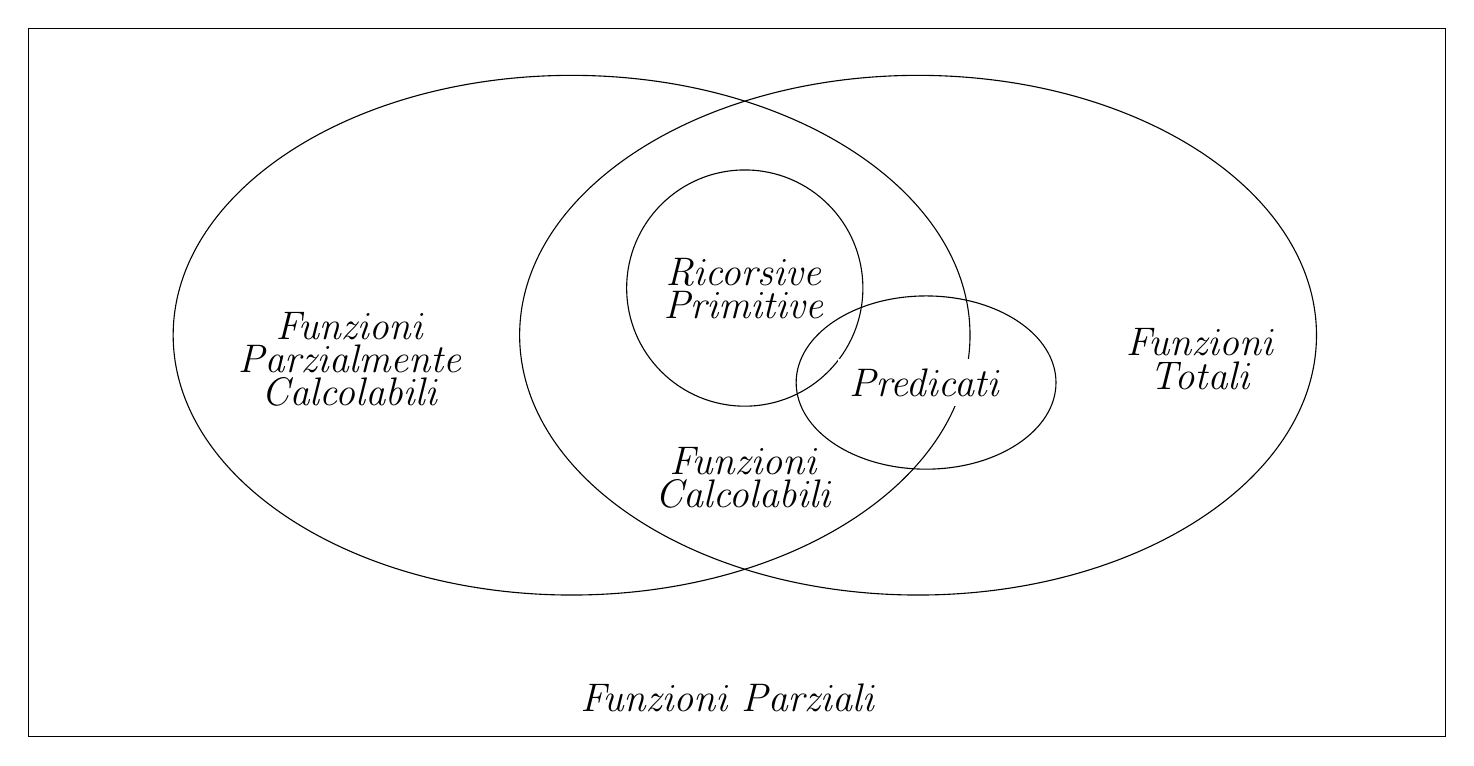
\begin{tikzpicture}
    % Define the size of the rectangle
    \draw[draw=black] (9.1, 6.2) rectangle ++(18, 9);

    % Calculate the center of the rectangle and move it on the y-axis
    \coordinate (center) at (16, 11.3);

    \begin{scope}
      % Create the first circle
      \draw[xscale=2.3, yscale=1.5] (center) circle (2.2cm);
    \end{scope}

    \begin{scope}
      % Calculate the position for the second circle relative to the center
      % Reduce the xshift to make the circles overlap more
      \coordinate (secondCircle) at ([xshift=4.4cm] center);

      % Create the second circle
      \draw[xscale=2.3, yscale=1.5] (secondCircle) circle (2.2cm);
    \end{scope}

    \begin{scope}
      % Calculate the position for the third circle relative to the center and move it on the y-axis
      \coordinate (thirdCircle) at ([xshift=2.2cm, yshift=0.6cm] center);

      % Create the third circle
      \draw (thirdCircle) circle (1.5cm);

      % Text inside the third circle
      \node[align=center, text width=5cm] at (thirdCircle) {\Large{\textit{Ricorsive}}\\ \Large{\textit{Primitive}}};
    \end{scope}

    \begin{scope}
      % Calculate the position for the fourth circle relative to the center and move it on the y-axis
      \coordinate (fourthCircle) at ([xshift=4.5cm, yshift=-0.6cm] center);

      % Create the fourth circle
      \draw[xscale = 1.5] (fourthCircle) circle (1.1cm);

      % Text inside the fourth circle
      \node[align=center, text width=2cm, fill=white] at (fourthCircle) {\Large{\textit{Predicati}}};
    \end{scope}

    % Text
    \node[align=center, xshift=13.2cm, yshift=11cm, inner color = white] {\Large{\textit{Funzioni}}\\ \Large{\textit{Parzialmente}} \\\Large{\textit{Calcolabili}}};
    \node[below] at (18, 7) {\Large{\textit{Funzioni Parziali}}};
    \node[align=center, xshift=24cm, yshift=11cm] {\Large{\textit{Funzioni}}\\\Large{\textit{Totali}}};
    \node[align=center, xshift=18.2cm, yshift=9.5cm] {\Large{\textit{Funzioni}}\\\Large{\textit{Calcolabili}}};
  \end{tikzpicture}
  \caption{Diagramma Riassuntivo sulle Funzioni Parziali}
\end{figure}

Abbiamo infatti visto come possano esistere \textit{Funzioni parzialmente calcolabili}, come la sottrazione fra due numeri, \textit{Funzioni Parziali non Calcolabili}, tra l'altro anche \textit{Totali} come \textbf{\textit{HALT}}, e \textit{Funzioni Totali Calcolabili}, come la somma fra due numeri.

Abbiamo poi visto come anche tra i predicati esistano \textit{Predicati Calcolabili} come il \textbf{predicato di uguaglianza} e predicati non calcolabili, considerando ad esempio sempre \textbf{\textit{HALT}}.

Abbiamo poi definito la classe delle \textit{Funzioni ricorsiva primitive}, di cui abbiamo visto esempi anche tra i predicati come la \textbf{funzione rilevatrice di zeri}.

Ci manca solo da analizzare il caso di una funzione che sia \textit{calcolabile}, ma che non appartenga alle funzioni \textit{ricorsive primitive}. Per mostrare ciò ci avvarremo della \textbf{funzione di Ackermann-Péter}.

\begin{generalbox}[colframe=azure-gradient-3!90!black]{Esempio di funzione calcolabile ma non Ricorsiva Primitiva}
  Funzione di Ackermann-Péter
  \begin{equation}
    A(x,y) = \begin{cases}
      y+1, & x=0\\
      A(x-1,1), & y=0\\
      A(x-1,A(x,y-1)), & \text{altrimenti}
    \end{cases}
  \end{equation}

  Per quanto si possa agilmente scrivere un S-programma che calcoli questa funzione, questa non è ricorsiva primitiva.

  Vediamo infine un esempio di calcolo di questa funzione per input \((2,1)\):
  \begin{equation}
      A(2,1) = A(1,A(2,0))
  \end{equation}

  Calcoliamo dunque separatamente \(A(2,0)\):
  \begin{equation}
    A(2,0) = A(1,1) = A(0,A(1,0)) = A(1,0) +1 = A(0,1) +1 = 3
  \end{equation}

  Avremo dunque:
  \begin{equation}
    A(2,1) = A(1,A(2,0))=A(1,3)=A(0,A(1,2))=A(1,2) + 1 = A(0,A(1,1)) + 1 = A(1,1) + 1 + 1 = 3 + 1 +1 = 5
  \end{equation}
\end{generalbox}


